
    %---------------------------------------------------------
    
    \section{The IMEX semi-implicit model}
    
    %---------------------------------------------------------

    \begin{frame}
		\frametitle{Why go semi-implicit?}
		\begin{itemize}
			\item ENVIT can rise sharply on "bad" elements
			\item Diffusive CFL condition does not account for ENVIT, resulting in unstable step size for ERK
			\item Implicit schemes are complex, and have issues with non-linear convection
			\item Semi-implicit: good compromise between stability, complexity and performance
		\end{itemize}
    \end{frame}
    
    \begin{frame}
    \frametitle{The IMEX scheme}
    
    \begin{columns}
    
    \column{0.5\textwidth}
    
    \begin{itemize}
        \item \textbf{IM}plicit stiff \textbf{EX}plicit non-stiff scheme (\cite{bib:cavaglieri})
        \item Assumes a stiff linear diffusive term and a non-stiff non-linear convective term
        \item Similar to a generic Runge-kutta model, but uses separate coefficients for handling stiff and non-stiff terms
        \item Stiff term is linear, or already linearized; no outer iteration is needed
        \item Multiple combinations of Implicit/Explicit tables available %\cite{cavaglieri}
    \end{itemize}
    
    \column{0.5\textwidth}
    
    \begin{align*}
        \frac{\partial u}{\partial t} + \mathbf{g}(u) + \mathbf{f}(u) = 0 \\
        \mathbf{f}(u) = A u
    \end{align*}
    
    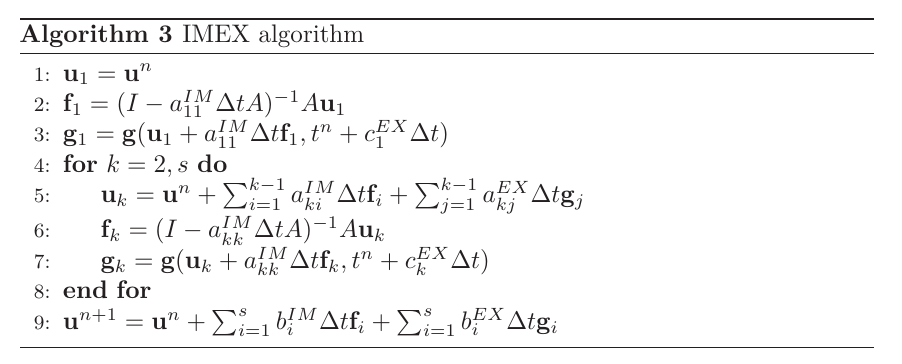
\includegraphics[width=\textwidth]{images/basic_imex.png}
    
    
    \end{columns}
    
    \end{frame}
    
    %---------------------------------------------------------
    
    \begin{frame}
    \frametitle{Stability properties}
    
    \begin{columns}
    
    \column{0.5\textwidth}
    
    \begin{itemize}
        \item Implicit terms are unconditionally stable, independent of the IMEX scheme adopted
        \item Explicit stability region dependent on the ERK scheme employed
    \end{itemize}
    
    \begin{block}{Remark}
        This effectively makes the time-step dependent only on the convective CFL condition, which is much more relaxed on fine meshes.
    \end{block}
    
    \column{0.5\textwidth}
    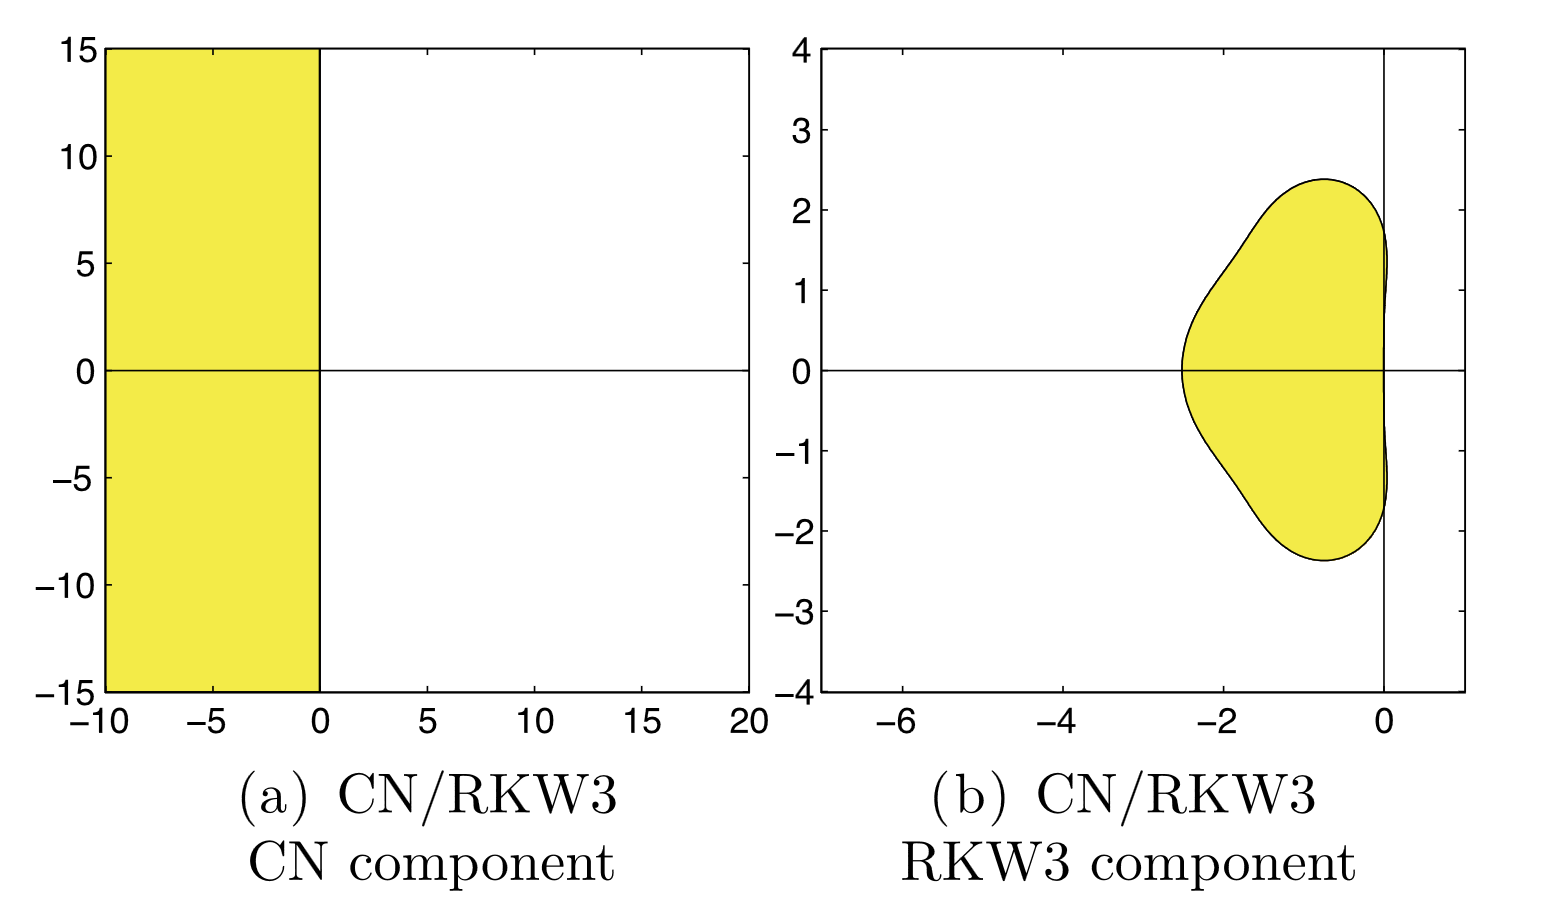
\includegraphics[width=1.1\textwidth]{images/imex_stab.png}
    
    \end{columns}
    
    \end{frame}
    
    %---------------------------------------------------------
    
    \begin{frame}
    \frametitle{Linear solver for the implicit terms}
    
    \begin{columns}
    
    \column{0.5\textwidth}
    
    \begin{itemize}
        \item \textbf{P}reconditioned \textbf{C}onjugate \textbf{G}radient
        \item Uses a diagonal matrix as preconditioner
        \item Simple and efficient GPU implementation
        \item Mixed precision implementation: dot products computed in FP64, but inputs and result stored in FP32
    \end{itemize}
    
    \begin{block}{Remark}
        The mixed precision aspect of the solver is crucial, as it enables the solver to be both performant on GPUs and accurate in key operations such as dot products over long arrays.
    \end{block}
    
    \column{0.5\textwidth}
    
    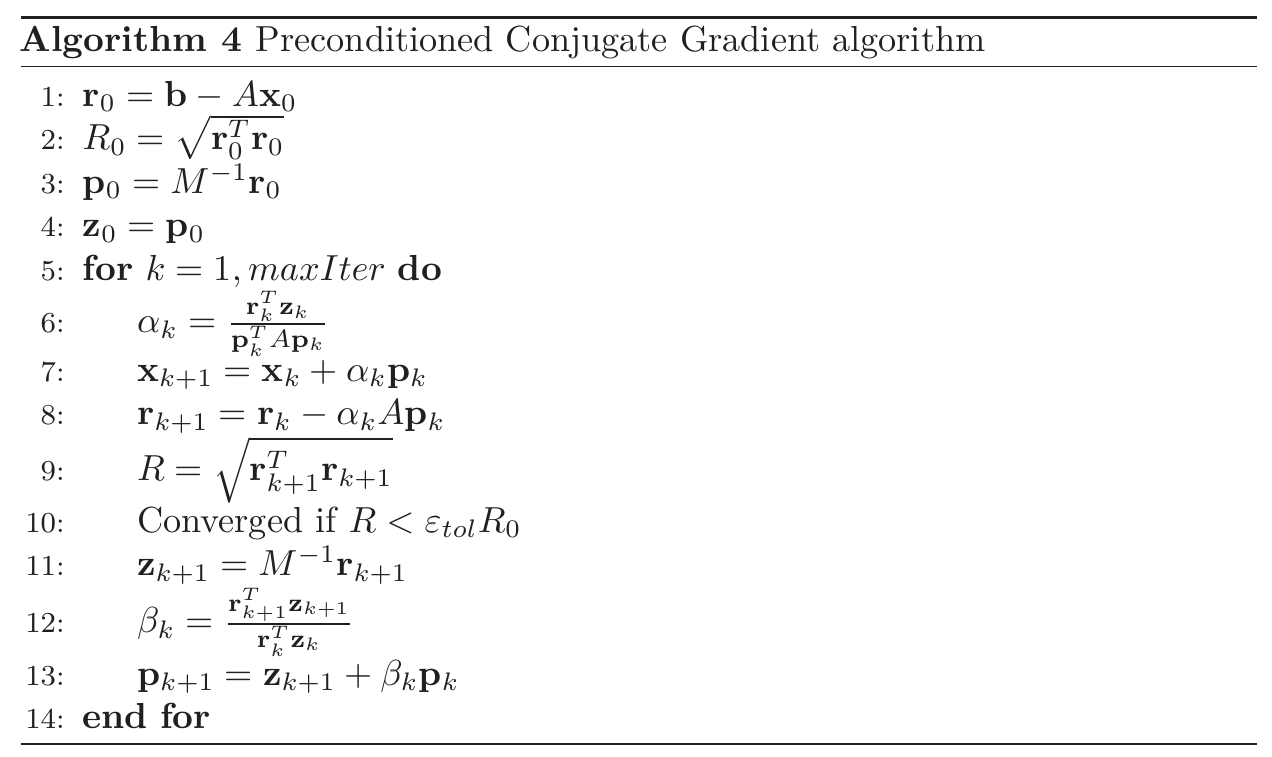
\includegraphics[width=1.1\textwidth]{images/pcg_basic.png}
    
    \end{columns}
    
    \end{frame}
    
    \begin{frame}
    \frametitle{IMEX: table of coefficients}
    
    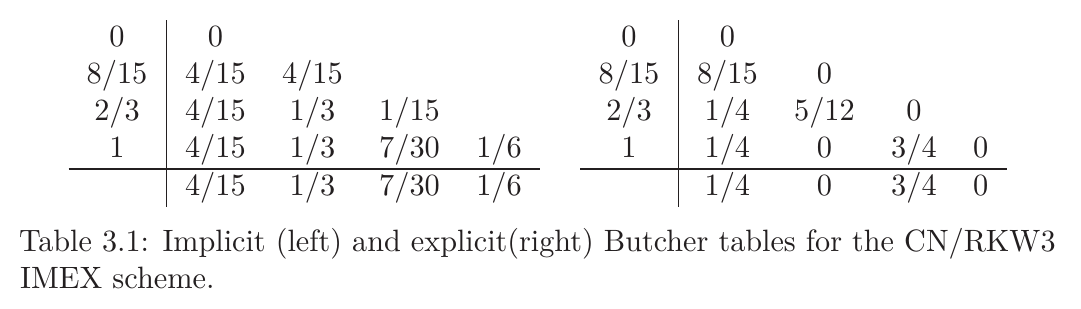
\includegraphics[width=1.0\textwidth]{images/imex_rkwcn.png}
    \end{frame}
    
    \begin{frame}
      \frametitle{IMEX implementation}
      
      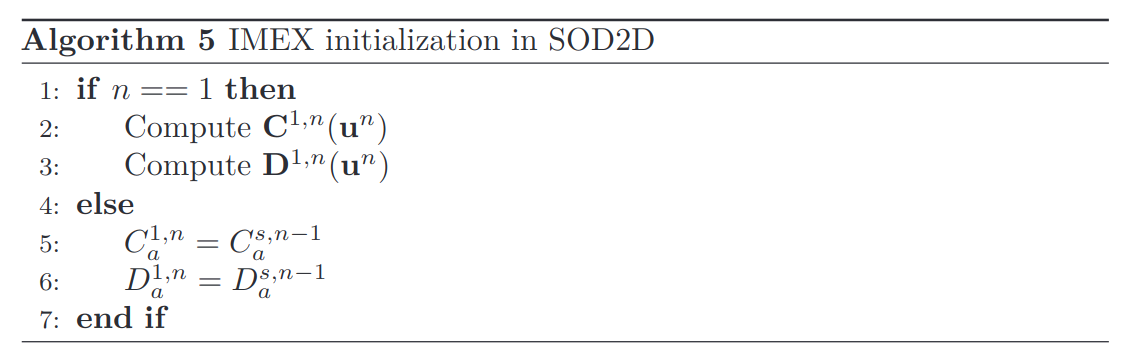
\includegraphics[width=0.95\textwidth]{images/imexSOD_init.png}
      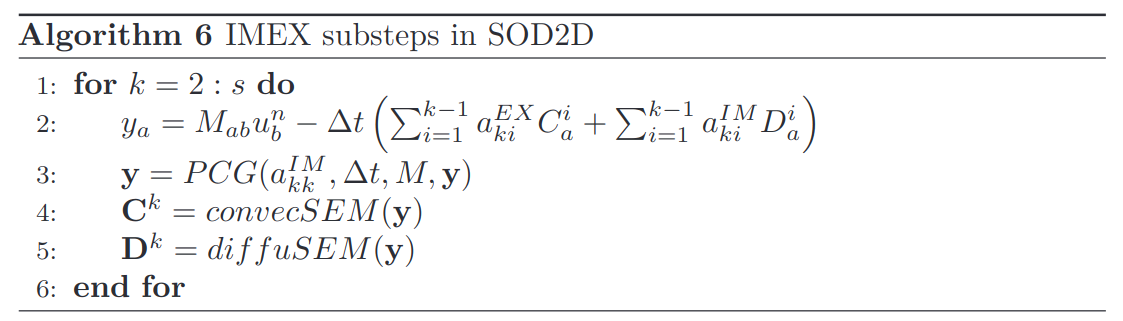
\includegraphics[width=0.95\textwidth]{images/imexSOD_steps.png}
      
    \end{frame}
      
    \begin{frame}
    \frametitle{Matrix-free PCG}
    
    \begin{columns}
    
    \column{0.5\textwidth}
    
    The implemented solver follows the algorithm shown, except that the matrix-vector products are substituted with calls to the SEM operator for the diffusive term.
    
    The preconditioner is the mass matrix of the SEM discretization, which is naturally diagonal.
    
    \column{0.5\textwidth}
    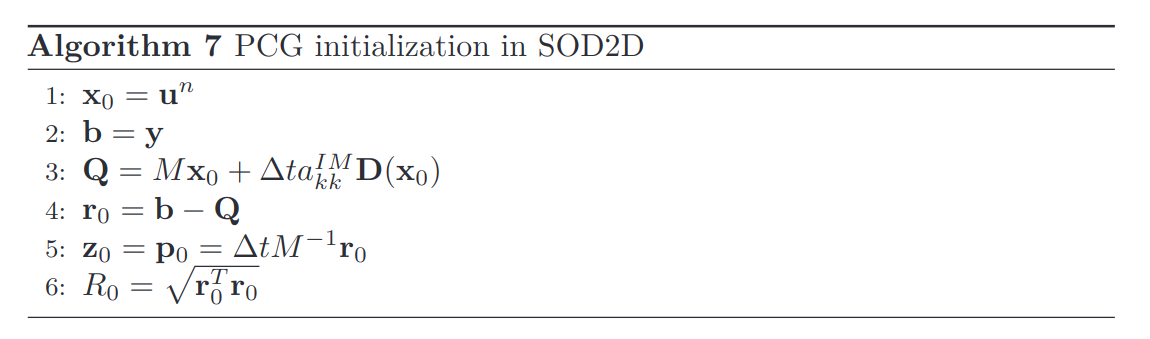
\includegraphics[width=1.1\textwidth]{images/pcgSOD_init.png}
    
    \begin{block}{Remark}
        Once the iterative process begins, the matrix-vector producs are computed as:
    
        \begin{align*}
            \mathbf{Q}  = M \mathbf{p_k} + \Delta t a^{IM}_{kk} \mathbf{D} (\mathbf{p_k})
    \end{align*}
    
    \end{block}
    
    \end{columns}
    
    \end{frame}